\chapter{Introducción}

\section{¿Qué es la materia condensada?}

\begin{itemize}
    \item Fases condensadas: aparecen cuando los sistemas f\'isicos est\'an formados por un n\'umero grande de elementos que interact\'uan fuertemente.
    \item Fases condensadas bastante conocidas: s\'olidos, l\'iquidos.
    \item Otras fases condensadas: superconductores, superfluidos, ferromagnetos, antiferromagnetos, condensados Bose-Einstein.
    \item Otras mesofases: cristales líquidos, membranas autoensambladas, geles, coloides, cristales, vidrios, etc.
\end{itemize}

Categorías de la física:
\begin{itemize}
    \item Teórico
    \item Experimental
    \item Fenomenológica
    \item Computacional
\end{itemize}

\subsection{De la física del estado sólido a la física de la materia condensada}

\begin{itemize}
    \item La física del estado sólido en los 30 (siglo XX):
    \begin{itemize}
        \item Cristalografía por Rayos X
        \item Difracción de electrones
        \item M cuántica + M estadística
    \end{itemize}
\end{itemize}

\subsection{Tipos de fuerzas}


\begin{itemize}
    \item Van der Waals
    \item Interacción electromagnética
    \item Interacción de intercambio
    \item Potencial de London
    \item Potencial de Lenard-Jones
\end{itemize}

\section{¿Qué estudia la materia condensada?}

Se vale de muchos métodos para estudiar la materia. 
\begin{itemize}
    \item Mecánica estadística
    \begin{itemize}
        \item Modelo de campo medio
        \item Movimiento Browniano
        \item Dinámica molecular
    \end{itemize}
    \item Mecánica cuántica
    \begin{itemize}
        \item Modelo de Hubbard (1963-1966)
        $$\hat{H}=-t\sum_{\langle i,j\rangle\sigma}\left(C_{i\sigma}^\dagger C_{j\sigma}+C_{j\sigma}^\dagger C_{i\sigma}\right)+U\sum_{i}n_{i\uparrow}n_{i\downarrow}$$
        Donde:
        \begin{itemize}
            \item $C_{i\sigma}^\dagger$: Operador bosónico de creación de partículas de espín $\sigma$ en la posición $i$.
            \item $C_{j\sigma}$: Operador bosónico de aniquilación de partículas de espín $\sigma$ en la posición $j$.
            \item $n_i$: Operador número en la posición $i$.
        \end{itemize}
    \end{itemize}
\end{itemize}

\textbf{Un mol} es $6.022E23$.

\subsection{Objetivo de la materia condensada}
\begin{itemize}
    \item El objetivo de la Física de la materia condensada es el entendimiento de las propiedades de grandes conjuntos de átomos y moléculas en términos de las interacciones entre ellas.
    \item Propiedades macroscópicas
    \begin{itemize}
        \item Temperatura
        \item Presión
        \item Volumen
        \item Energía de enlace
        \item Opacidad
    \end{itemize}
    \item De lo más notable de la física de la materia condensada, es el poder explicar la fenomenología de un sistema que surge de un Hamiltoniano relativamente simple.
\end{itemize}

\subsection{Hitos de la física de la materia condensada}

\begin{itemize}
    \item Efecto fotoeléctrico (Einstein, 1905)
    \item Capacidad Calorífica (Einstein, 1907)
    \item Ferromagnetismo (Weiss, 1907)
    \item Licuefacción de He @ 4.1K (Kemerling Onnes, 1908)
    \item Superconductividad (Kamerling Onnes, 1911) 
    \item Difracción de Rayos X (Von Laue, 1912)
    \item Cuantización de las vibraciones de una red cristalina (Max Born, 1912)
    \item Corrección de la aproximación de la capacidad calorífica (Debye, 1912)
    \item Ecuación de Schrodinger (Schrodinger, 1926)
    \item Principio de exclusión de Pauli (Pauli, 1926)
    \item Aproximación Born-Oppenheimer (1927) Desacoplan dinámicas de núcleos y electrones.
    \item Descripción cuántica del modelo de electrones libres (Sommerfeld, 1928)
\end{itemize}

\subsection{Materia Blanda y Materia Sólida}

Orden (desorden) estadístico:

\begin{align*}
    \text{Entropía}\\
    S=-k\log\omega
\end{align*}

\begin{figure}[H]
    \centering
    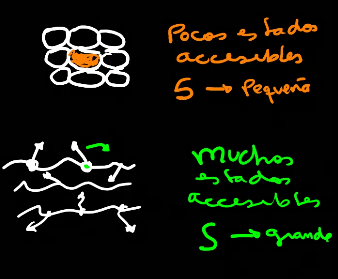
\includegraphics[width=0.4\textwidth]{Graficas/Jul27-1.png}
    \caption{Sólidos ordenados, líquidos desordenados}
    \label{fig:SolLiq}
\end{figure}

Tres categorías:

\begin{enumerate}
    \item Orden de largo alcance
    \item Orden de corto alcance
    \item Desorden
\end{enumerate}


\textbf{Materia blanda:}

\begin{itemize}
    \item Escalas de longitud: Desde escalas atómicas a escalas macroscópicas.
    \item Fluctuaciones
    \item Autoreorganización


\item\textbf{Macroscópicas}

\begin{itemize}
    \item Polímeros
    \item Interfaces
\end{itemize}

\item\textbf{Microscópicas}

\begin{itemize}
    \item Coloides
    \item Geles 
    \item Cristales líquidos
\end{itemize}

\end{itemize}

\subsubsection*{Fluctuaciones y Movimiento Browniano}

\begin{itemize}
    \item Partes pequeñas que tienen movimiento aleatorio
    \item Fluctuaciones térmicas
\end{itemize}

\subsection{Materia sólida} 

Cristalografía clásica: Sistemas que se representan como puntos con patrons específicos.
\begin{itemize}
    \item Grupos de traslación (redes Bravais)
    \item Traslación y simetría (grupos de Schontlis)
\end{itemize}


\subsection{Fases de la materia}

\begin{tabular*}{0.8\textwidth}{l|rl}
             & Ordenadas & No ordenadas\\
             \hline
     Clásica & Hielo de agua & Agua líquida\\
     Cuántica & Ferromagnética\\
                & Antiferromagnética\\
\end{tabular*}

\subsection{Conjuntos de puntos:}

\begin{itemize}
    \item Conjunto unitario: tiene un solo elementos.
    \item La union contable de conjuntos unitarios suma un conjunto de puntos.
    \item Un conjunto de puntos, $\Lambda\subset \mathbb{R}^d$, es un conjunto discreto si $x\in \Lambda$ tiene una vecindad abierta $U=U(x)\subset \mathbb{R}^d$ que no tiene ningún elemento de $\Lambda$.
    \item Para cada $x\in\Lambda$, exite un radio de empaquetamiento $r>0$ tal que $B(r)$ es una hiperesfera de radio $r$ tal que $B_r(x) \cap \Lambda=\{x\}$.
    \item Por otro lado, $\Lambda$ es uniformemente discreto si hay una vecindad abierta, $U$, de $0\in\mathbb{R}^d$ tal que $(x+U)\cap(y+U)=\emptyset$. Se cumple para todo $x,y\in\Lambda$ la suma y diferencia de Minkowski para dos conjuntos $U\pm V:=\left\{u\pm v \lvert u \in U,v\in V\right\}$
    \item Para un conjunto discreto se tiene una distancia mínima entre puntos. Los subconjuntos de $\mathbb{Z}$ son uniformemente discretos. Pero podemos construir conjuntos discretos no uniformes, por ejemplo: $A=\left\{\frac{1}{n}\lvert n\in \mathbb{N}\right\}$
    \item Un conjunto $\Lambda$ es localmente finito, si para todos los conjuntos $K\subset \mathbb{R}^d$, $K\cap\Lambda$ es un conjunto finito o $\emptyset$. 
    ``Cuando $\Lambda$ es un conjunto de puntos, también es localmente finito si y solo si es discreto y cerrado.'' Además, $\Lambda$ es relativamente denso si existe un conjunto compacto $K\subset \mathbb{R}^d$ tal que $\Lambda+K=\mathbb{R}^d$.
    \item Un conjunto de puntos $\Lambda\subset\mathbb{R}^d$ es un conjunto de Delone (Delany), ``un Delone'' si es uniformemente discreto y relativamente denso.
    \item Para cualquier conjunto de Delone, $\Lambda\subset \mathbb{R}^d$ se puede elegir un radio de empaquetamiento $r$ y otro de ``recubrimiento'', $R$ tal que $U=B_r(0)$ (hiperesfera) y $K=\overline{B_R(0)}$ son vecindades apropiadas para confinar $\Lambda$.
    \item Un conjunto de puntos $\Lambda\subset \mathbb{R}^d$ es un conjunto de Meyer, ``un Meyer'', si $\Lambda$ es relativamente denso y $\Lambda-\Lambda$ es uniformemente discreto.
    \item Todos los conjuntos de Meyer son de Delone, pero no todos los conjuntos de Delone son de Meyer.
\end{itemize}

\textbf{Por ejemplo:}

\begin{align*}
    \Lambda&=\left\{n+\frac{1}{n}\rvert n \in \mathbb{Z}\backslash 0\right\}\\
        &=\left\{2,2\frac{1}{2},3\frac{1}{3},\cdots\right\}
\end{align*}

\begin{itemize}
    \item Es uniformemente discreto.
    \item Tiene un radio de empaquetamiento $r=1/4$
    \item Es relativamente denso
    \item Radio de recubrimiento $R=2$
\end{itemize}

Es un conjunto de Delone.
No es un conjunto de Meyer.

\begin{itemize}
    \item Un conjunto de puntos $\Gamma \subset \mathbb{R}^d$ son puntos de red (grid). O simplemente una red en $\mathbb{R}^d$ si existen $d$ vectores $\vec{b}_1,\cdots,\vec{b}_d$ tal que
    $$
        \Gamma=\mathbb{Z}b_1\oplus\cdots\oplus\mathbb{Z}b_d:=\left\{\sum_{i=1}^dm_ib_i\lvert\forall m_i\in\mathbb{Z}\right\}
    $$
    y que además, si $\mathbb{R}^d$ es generado por $\left\{b_1,\cdots,b_d\right\}$ es una base de la red $\Gamma$.
\end{itemize}